% Reading the Trail: Off-Road Terrain Analysis with Deep Convolutional Networks
% Build: latexmk -pdf main.tex   (run inside paper/)
%
% Each section lives in sections/<name>.tex so team members can edit in parallel.
% Result-dependent text is marked with \todo{...} (inline note) or \tbd (a number
% still to be filled in). Search for "\todo" and "\tbd" before submission; setting
% \finaltrue below turns any leftover placeholder into a compile error.
\documentclass[conference]{IEEEtran}

\usepackage[utf8]{inputenc}
\usepackage[T1]{fontenc}
\usepackage{amsmath,amssymb}
\usepackage{graphicx}
\usepackage{booktabs}
\usepackage{multirow}
\usepackage{array}
\usepackage{siunitx}
\usepackage{xcolor}
\usepackage{tikz}
\usetikzlibrary{arrows.meta,positioning,fit,backgrounds,calc,shapes.geometric}
\usepackage[hidelinks]{hyperref}
\usepackage{cite}

% ---------------------------------------------------------------------------
% Placeholder macros (visible in the PDF).
\newif\iffinal
\finalfalse
\iffinal
  \newcommand{\todo}[1]{\errmessage{Unresolved TODO: #1}}
  \newcommand{\tbd}{\errmessage{Unresolved TBD number}}
\else
  \newcommand{\todo}[1]{{\color{red!75!black}\textbf{[TODO:~#1]}}}
  \newcommand{\tbd}{{\color{red!75!black}\textbf{??}}}
\fi
% A framed box standing in for a figure that does not exist yet.
\newcommand{\placeholderfig}[2]{%
  \fbox{\parbox[c][#1][c]{0.95\linewidth}{\centering\color{red!75!black}%
  \textbf{[FIGURE PLACEHOLDER]}\\[2pt]\footnotesize #2}}}

% Notation.
\newcommand{\etal}{et~al.}
\newcommand{\miou}{mIoU}
\newcommand{\eg}{e.g.,\ }
\newcommand{\ie}{i.e.,\ }

\begin{document}

\title{Reading the Trail: Off-Road Terrain Analysis\\with Deep Convolutional Networks}

\author{%
\IEEEauthorblockN{Callen Nash}
\IEEEauthorblockA{\textit{Model \& documentation lead}\\
Colorado School of Mines\\
Golden, CO, USA}
\and
\IEEEauthorblockN{Xander Navojosky}
\IEEEauthorblockA{\textit{Data \& evaluation lead}\\
Colorado School of Mines\\
Golden, CO, USA}
}

\maketitle

% Abstract: 100-150 words (Requirements.md).
\begin{abstract}
Off-road robots must tell drivable ground from water, logs, and dense
vegetation, yet the classes that matter most for safety are among the rarest.
On the RUGD dataset we compare U-Net and DeepLabV3+ with ImageNet-pretrained
ResNet encoders and five training losses, selecting models on validation
only. DeepLabV3+/ResNet-50 with cross-entropy plus Dice reaches 37.7\% test
mIoU and 60.0\% over six traversability groups. Pretraining adds about six
points and Dice terms about three, while a deeper encoder and focal loss stay
within seed noise, and median-frequency weighting hurts. Part of the apparent
gains came from scoring classes absent from validation. One unseen creek
scene accounts for 80\% of test errors: its shallow water is labeled
drivable ground. Zero-shot on RELLIS-3D, group mIoU falls to 43.4\%, with
ground and water transferring worst.
\end{abstract}


\section{Introduction and Motivation}
\label{sec:intro}

Most work on visual perception for autonomous driving targets paved urban
streets, where lane markings, curbs, and signs give a model strong geometric
and semantic structure~\cite{cordts2016cityscapes}. Off-road terrain offers
none of this. Boundaries between grass, mulch, and gravel are irregular and
often ambiguous, lighting changes abruptly under tree cover, and a camera on a
small vehicle shakes and blurs as it crosses rough
ground~\cite{wigness2019rugd}. Yet many high-value uses of autonomy happen
off-road: search-and-rescue and disaster-relief robots, agricultural and
forestry vehicles, planetary rovers, and military logistics. For these
systems, distinguishing drivable dirt from standing water or a fallen log is a
central perception problem, and a mistake can leave a vehicle stuck or damaged.
The same capability could also support driver-assist cameras on consumer
off-road vehicles that warn about water crossings, loose rock, or obstacles
before the driver commits to a line.

We treat terrain understanding as \emph{semantic segmentation}: assign each
pixel of a forward-facing camera image one of the 24 terrain and object
classes of the RUGD dataset~\cite{wigness2019rugd}. Two properties make this
harder than urban segmentation. First, the label distribution is extremely
skewed: in the RUGD training split, \emph{tree} and \emph{grass} cover 63\% of non-void
labeled pixels, while \emph{water}, \emph{rock}, and \emph{log} together
cover under 0.8\% (Fig.~\ref{fig:classfreq}), even though these rare classes
are the ones most relevant to safe driving. Second, RUGD is small (7,436
annotated frames from 18 video sequences) and its frames are strongly
correlated in time, so careless splitting would leak near-duplicate frames
between training and test.

This project asks three questions that transfer beyond off-road driving:
(i)~how much do the decoder design and the encoder depth matter when both
start from ImageNet-pretrained weights; (ii)~which class-imbalance loss most
improves accuracy on rare, safety-relevant classes without sacrificing overall
accuracy; and (iii)~how much does ImageNet pretraining help on scenes far from
its training distribution. As a stretch goal, we test how a RUGD-trained model
transfers to RELLIS-3D~\cite{jiang2021rellis}, which was recorded with a
different vehicle in a different environment.

Our contributions are:
\begin{itemize}
  \item A controlled comparison of U-Net~\cite{ronneberger2015unet} and
        DeepLabV3+~\cite{chen2018deeplabv3plus} with ImageNet-pretrained
        ResNet-18/50 encoders~\cite{he2016resnet} on RUGD, changing one factor
        per experiment and selecting models on the validation split only. We
        find that \todo{architecture/encoder finding}.
  \item A comparison of four imbalance-aware losses (median-frequency weighted
        cross-entropy, Dice, focal, and cross-entropy plus Dice) against plain
        cross-entropy, reported per class with emphasis on rare,
        safety-relevant terrain. \todo{loss finding, e.g., which loss improves
        water/log/rock IoU and at what cost to mIoU}.
  \item An ablation of ImageNet pretraining and a multi-seed estimate of
        run-to-run variance for the two strongest configurations.
        \todo{pretraining gap and seed std}.
  \item An error analysis built on the normalized confusion matrix, worst-frame
        galleries, and a six-group traversability evaluation, together with a
        documented account of the data-integrity issues we found in RUGD, such
        as a class that appears only in the test split and a validation split
        that lacks four classes.
        \todo{RELLIS-3D cross-dataset result, if completed.}
  \item An open, configuration-driven pipeline in which every experiment is a
        YAML file and every model-selection decision is made automatically
        from validation scores and logged.
\end{itemize}

\section{Related Work}
\label{sec:related}

\subsection{Off-Road Segmentation Datasets and Benchmarks}

\textbf{RUGD.} Wigness \etal{}~\cite{wigness2019rugd} released RUGD, more than
7,000 frames from video sequences recorded by a small unmanned ground robot
whose camera sits under 25\,cm above the ground, densely annotated with 24
classes. They partition the 18 sequences into train, validation, and test
splits, and deliberately place \emph{creek} (the only sequence with substantial
rock-bed terrain) and \emph{trail-7} (heavy motion blur) in the test split. Their
baselines all use a ResNet-50 encoder with PSPNet, UPerNet, or simpler
decoders, trained at $688\times555$. These reach 35.7--36.7\% mIoU on
validation but only 31.8--32.2\% on test (24-class mIoU; Tables~II and~III
of~\cite{wigness2019rugd}). Every baseline scores 0.0 IoU on \emph{bridge}
(Table~V of~\cite{wigness2019rugd}). We follow their sequence split exactly and
use their test mIoU as a historical reference point, not as a directly
comparable number, since our resolution, class averaging, and training budget
differ (Section~\ref{sec:methods}).

\textbf{RELLIS-3D.} Jiang \etal{}~\cite{jiang2021rellis} recorded RELLIS-3D with
a larger off-road vehicle on a Texas A\&M University campus. It provides
6,235 annotated camera images and 13,556 annotated LiDAR scans. On their image
test split, HRNetV2+OCR and Gated-SCNN reach only 51.55\% and 52.92\% mIoU
(Table~II of~\cite{jiang2021rellis}). The authors attribute the low scores to
severe class imbalance and unclear terrain boundaries. RELLIS-3D also contains
classes that RUGD lacks, such as \emph{mud}, \emph{puddle}, and \emph{rubble},
which motivates the shared group-level class map we use for the cross-dataset
test.

\textbf{Off-road methods.} GA-Nav~\cite{guan2022ganav} merges the fine classes
of both datasets into six navigability groups and adds a group-wise attention
mechanism to a transformer backbone. Under that grouping, GA-Nav reports
89.08\% mIoU on RUGD and 74.44\% on RELLIS-3D, compared with 55.88\% and
62.27\% for its DeepLabv3+ baseline (Table~V of the arXiv version
of~\cite{guan2022ganav}). Their groups (smooth, rough, bumpy, forbidden,
obstacle, background) differ from our six traversability groups, so these
figures show the gain from coarse grouping and are not directly comparable to
our group mIoU.

\subsection{Architectures and Pretraining}

U-Net~\cite{ronneberger2015unet} pairs a contracting encoder with a symmetric
expanding decoder and concatenates encoder features into the decoder at every
scale, which preserves fine spatial detail.
DeepLabV3+~\cite{chen2018deeplabv3plus} instead relies on atrous spatial
pyramid pooling (ASPP)~\cite{chen2017deeplabv3}, parallel dilated convolutions
that capture multi-scale context at reduced resolution, and adds a lightweight
decoder with a single low-level skip connection to refine boundaries. Both are
commonly paired with residual encoders~\cite{he2016resnet} pretrained on
ImageNet~\cite{deng2009imagenet}, which speeds convergence and helps when
labeled data is scarce. How well that transfer holds for low-viewpoint
natural terrain is one of the questions we test.

\subsection{Losses for Class Imbalance}

Weighted cross-entropy rescales each pixel's loss by a per-class weight. With
median-frequency balancing~\cite{eigen2015predicting}, the weight is the
median class frequency divided by the frequency of the pixel's class. Dice
loss~\cite{milletari2016vnet} directly optimizes a soft overlap measure that
is insensitive to how many pixels a class occupies. Focal
loss~\cite{lin2017focal} multiplies the cross-entropy term by
$(1-p_t)^\gamma$, which down-weights well-classified examples so that training
focuses on hard ones. Combining cross-entropy with Dice is a common way to
keep the stable gradients of the former while adding the class-balancing
effect of the latter. We compare all four under a fixed architecture.

\section{Methods}
\label{sec:methods}

Fig.~\ref{fig:arch} summarizes the pipeline shared by all experiments. Every
experiment is defined by one YAML file that inherits from a common base
configuration, so runs differ only in the factors listed in
Table~\ref{tab:protocol}.

\begin{figure*}[t]
  \centering
  \resizebox{\textwidth}{!}{% Architecture diagram (fig:arch). Self-contained tikzpicture: needs tikz with
% libraries arrows.meta, positioning, fit, backgrounds, calc.
% Included by main.tex (scaled to \textwidth) and by architecture_standalone.tex (PNG export).
\begin{tikzpicture}[
  font=\footnotesize,
  >={Stealth[length=2.2mm]},
  flow/.style={->, thick, draw=black!75},
  skip/.style={->, thick, draw=orange!80!black},
  lowskip/.style={->, thick, draw=violet!80!black},
  box/.style={draw=black!70, rounded corners=2pt, align=center, inner sep=3pt},
  enc/.style={box, draw=blue!55!black, fill=blue!10, minimum width=3.0cm, minimum height=0.62cm, font=\scriptsize},
  encdim/.style={enc, draw=blue!30, fill=blue!4, text=black!55},
  udec/.style={box, draw=orange!75!black, fill=orange!12, minimum width=2.9cm, minimum height=0.62cm, font=\scriptsize},
  ddec/.style={box, draw=violet!75!black, fill=violet!10, minimum height=0.62cm, font=\scriptsize},
  head/.style={box, draw=black!60, fill=black!6, minimum height=0.62cm, font=\scriptsize},
  panel/.style={draw=black!35, rounded corners=4pt, inner sep=6pt},
  ptitle/.style={font=\small\bfseries, anchor=south west},
  lbl/.style={font=\scriptsize, text=black!70},
]

% =====================================================================
% TOP: shared pipeline
% =====================================================================
\begin{scope}[yshift=0.45cm]
  % Input "image" icon: sky / tree line / trail.
  \begin{scope}[shift={(0,-0.75)}]
    \fill[blue!30] (0,0.95) rectangle (1.8,1.5);
    \fill[green!45!black!70] (0,0.55) -- (0.3,1.05) -- (0.55,0.8) -- (0.85,1.15) -- (1.15,0.85) -- (1.45,1.1) -- (1.8,0.8) -- (1.8,0.55) -- cycle;
    \fill[green!55!black!45] (0,0) rectangle (1.8,0.58);
    \fill[brown!55] (0.6,0) -- (0.85,0.58) -- (0.98,0.58) -- (1.35,0) -- cycle;
    \draw[black!70] (0,0) rectangle (1.8,1.5);
  \end{scope}
  \node[lbl, align=center, anchor=north] (inlbl) at (0.9,-0.8) {RGB input\\$3\times384\times384$\\ImageNet-normalized};
  \coordinate (inR) at (1.8,0);

  % Encoder trapezoid (wide input side, narrow deep side).
  \draw[draw=blue!55!black, fill=blue!10, rounded corners=1pt]
    (3.0,-1.1) -- (3.0,1.1) -- (5.75,0.6) -- (5.75,-0.6) -- cycle;
  \coordinate (encW) at (3.0,0); \coordinate (encE) at (5.75,0);
  \node[align=center, font=\footnotesize, inner sep=0pt] (enc) at (4.3,0) {\textbf{Encoder}\\ResNet-18 / -50\\ImageNet init.\\{\scriptsize features $\tfrac12\ldots\tfrac1{32}$}};
  \draw[flow] (inR) -- (encW);

  % Decoder choices.
  \node[udec, minimum width=3.1cm, font=\footnotesize] (dU) at (8.55,0.52) {\textbf{(a) U-Net decoder}\\skips at every scale};
  \node[ddec, minimum width=3.1cm, font=\footnotesize] (dD) at (8.55,-0.62) {\textbf{(b) DeepLabV3+ decoder}\\ASPP @ $\tfrac1{16}$ + skip @ $\tfrac14$};
  \node[lbl, font=\scriptsize\itshape] at (8.55,-0.05) {or};
  \node[draw=black!40, dashed, rounded corners=3pt, fit=(dU)(dD), inner sep=3pt] (dec) {};
  \draw[flow] (encE) -- (encE -| dec.west);

  % Logits.
  \node[head, minimum width=2.1cm, minimum height=1.0cm, font=\footnotesize] (logit) at (12.0,0) {\textbf{Logits}\\$25\times384\times384$};
  \draw[flow] (dec.east) -- (logit.west);

  % Training loss and evaluation.
  \node[box, draw=red!60!black, fill=red!6, text width=4.15cm, font=\scriptsize, anchor=west] (loss) at (13.75,0.5)
    {\textbf{Training loss} (one per run)\\CE $\cdot$ weighted CE (median-freq.)\\Dice $\cdot$ Focal ($\gamma{=}2$) $\cdot$ CE+Dice\\void pixels ignored};
  \node[box, draw=green!45!black, fill=green!7, text width=4.15cm, font=\scriptsize, anchor=west] (eval) at (13.75,-0.72)
    {\textbf{Evaluation}: argmax (void masked)\\per-class IoU, mIoU, 6-group IoU};
  \draw[flow] (logit.east) -- ++(0.25,0) |- (loss.west);
  \draw[flow] (logit.east) -- ++(0.25,0) |- (eval.west);
\end{scope}

% =====================================================================
% Shared helper geometry for the two detail panels.
%   rows: y(1/1)=-2.75, y(1/2)=-3.5, y(1/4)=-4.25, y(1/8)=-5.0, y(1/16)=-5.75, y(1/32)=-6.5
% =====================================================================
\def\yA{-2.75}\def\yB{-3.5}\def\yC{-4.25}\def\yD{-5.0}\def\yE{-5.75}\def\yF{-6.5}

% =====================================================================
% BOTTOM LEFT: (a) U-Net
% =====================================================================
\begin{scope}[xshift=0cm]
  \node[lbl] (uin) at (1.6,\yA) {input $384^2$};
  \node[enc] (u1) at (1.6,\yB) {stem\enspace$\tfrac12$\enspace 64 | 64};
  \node[enc] (u2) at (1.6,\yC) {layer1\enspace$\tfrac14$\enspace 64 | 256};
  \node[enc] (u3) at (1.6,\yD) {layer2\enspace$\tfrac18$\enspace 128 | 512};
  \node[enc] (u4) at (1.6,\yE) {layer3\enspace$\tfrac1{16}$\enspace 256 | 1024};
  \node[enc] (u5) at (1.6,\yF) {layer4\enspace$\tfrac1{32}$\enspace 512 | 2048};
  \foreach \a/\b in {uin/u1,u1/u2,u2/u3,u3/u4,u4/u5} \draw[flow] (\a) -- (\b);

  \node[udec] (ud1) at (6.45,\yE) {up$\times$2, concat, 2$\times$conv\enspace 256};
  \node[udec] (ud2) at (6.45,\yD) {up$\times$2, concat, 2$\times$conv\enspace 128};
  \node[udec] (ud3) at (6.45,\yC) {up$\times$2, concat, 2$\times$conv\enspace 64};
  \node[udec] (ud4) at (6.45,\yB) {up$\times$2, concat, 2$\times$conv\enspace 32};
  \node[udec] (ud5) at (6.45,\yA) {up$\times$2, 2$\times$conv\enspace 16};
  \foreach \a/\b in {ud1/ud2,ud2/ud3,ud3/ud4,ud4/ud5} \draw[flow] (\a) -- (\b);
  \draw[flow] (u5.east) -| (ud1.south);

  \foreach \e/\d in {u1/ud4,u2/ud3,u3/ud2,u4/ud1} \draw[skip] (\e.east) -- (\d.west);
  \node[lbl, text=orange!70!black, anchor=north] at ($(u4.east)!0.5!(ud1.west)+(0,-0.03)$) {skips};

  \node[head] (uh) at (9.45,\yA) {3$\times$3 conv\\$\to$ 25};
  \draw[flow] (ud5) -- (uh);
\end{scope}
\node[panel, fit=(uin)(u5)(ud5)(uh)(ud1)] (pa) {};
\node[ptitle] at (pa.north west) {(a) U-Net};

% =====================================================================
% BOTTOM RIGHT: (b) DeepLabV3+
% =====================================================================
\begin{scope}[xshift=11.0cm]
  \node[lbl] (din) at (1.6,\yA) {input $384^2$};
  \node[encdim] (d1) at (1.6,\yB) {stem\enspace$\tfrac12$\enspace 64 | 64};
  \node[enc] (d2) at (1.6,\yC) {layer1\enspace$\tfrac14$\enspace 64 | 256};
  \node[encdim] (d3) at (1.6,\yD) {layer2\enspace$\tfrac18$\enspace 128 | 512};
  \node[encdim] (d4) at (1.6,\yE) {layer3\enspace$\tfrac1{16}$\enspace 256 | 1024};
  \node[enc] (d5) at (1.6,\yF) {layer4\enspace$\tfrac1{16}$ (dilated)\enspace 512 | 2048};
  \foreach \a/\b in {din/d1,d1/d2,d2/d3,d3/d4,d4/d5} \draw[flow] (\a) -- (\b);

  \node[ddec, text width=2.3cm, anchor=west] (aspp) at (4.4,\yF)
    {\textbf{ASPP} @ $\tfrac1{16}$: 1$\times$1, rates 12/24/36, image pool $\to$ 256};
  \draw[flow] (d5.east) -- (aspp.west);

  \node[ddec, anchor=west] (low) at (4.4,\yC) {1$\times$1 conv\enspace 48};
  \draw[lowskip] (d2.east) -- (low.west);
  \node[lbl, text=violet!75!black, anchor=south] at ($(d2.east)!0.5!(low.west)+(0,0.05)$) {skip};

  \node[ddec, text width=1.35cm, anchor=west] (fuse) at (6.7,\yC) {concat, 3$\times$3 sep.\ conv 256};
  \draw[flow] (low.east) -- (fuse.west);
  \draw[flow] (aspp.east) -| node[pos=0.75, lbl, right, align=left] (uplbl) {bilinear\\up$\times$4\\($\tfrac1{16}\!\to\!\tfrac14$)} (fuse.south);

  \node[head] (dh) at (fuse.north |- 0,\yA) {1$\times$1 conv $\to$ 25, up$\times$4};
  \draw[flow] (fuse.north) -- (dh.south);
\end{scope}
\node[panel, fit=(din)(d5)(aspp)(dh)(fuse)(uplbl)] (pb) {};
\node[ptitle] at (pb.north west) {(b) DeepLabV3+};

% Legend line under the panels.
\node[lbl, anchor=north west, font=\scriptsize] at ($(pa.west |- pb.south)+(0,-0.08)$)
  {Encoder blocks: name, resolution, output channels for ResNet-18 | ResNet-50. Pale blocks: computed but not used by the decoder.};
\end{tikzpicture}
}
  \caption{Shared segmentation pipeline. Top: a $384\times384$ RGB frame is
  encoded by an ImageNet-pretrained ResNet-18 or ResNet-50, decoded by U-Net
  or DeepLabV3+, and mapped to 25 logits per pixel (24 RUGD classes plus
  \emph{void}, which is ignored in the loss and never predicted). Each
  experiment trains with exactly one loss variant. Bottom left: the U-Net
  decoder concatenates encoder features at every scale from $1/16$ to $1/2$.
  Bottom right: DeepLabV3+ dilates the last ResNet stage (output stride 16),
  applies ASPP, and fuses the result with a single $1/4$-scale skip connection.
  Channel counts are given for ResNet-18 / ResNet-50.}
  \label{fig:arch}
\end{figure*}

\subsection{Data and Splits}
\label{sec:data}

RUGD~\cite{wigness2019rugd} provides 7,436 annotated $688\times550$ frames from
18 video sequences. We use the official sequence-level split
(Table~\ref{tab:data}): no sequence appears in more than one split, so
near-identical consecutive frames cannot leak from training into evaluation. The
sequence assignment matches Table~I of~\cite{wigness2019rugd}. A split-check
script counts 4,779\,/\,733\,/\,1,924 frames in the released data. The paper's
table prints 4,759 and 1,964 for train and test, which sum to 20 more frames than
the 7,436 released. We use the counts from the released files.

\begin{table}[t]
  \centering
  \caption{RUGD sequence-level split used in all experiments.}
  \label{tab:data}
  \footnotesize
  \begin{tabular}{@{}l p{4.3cm} r@{}}
    \toprule
    Split & Sequences & Frames \\
    \midrule
    Train & park-2, trail, trail-3, -4, -6, -9, -10, -11, -12, -14, -15, village & 4,779 \\
    Val   & park-8, trail-5 & 733 \\
    Test  & creek, park-1, trail-7, trail-13 & 1,924 \\
    \bottomrule
  \end{tabular}
\end{table}

\textbf{Label decoding.} RUGD labels are color-coded RGB images. We decode them
to integer class indices with a 24-bit color lookup table built from the
dataset's own colormap file (25 entries: \emph{void} plus 24 classes). Any
color not in the table maps to an ignore index. \emph{Void} pixels are also
mapped to the ignore index, so they contribute to neither loss nor metrics, and
the void logit is masked out at prediction time.

\textbf{Class statistics.} Pixel frequencies on the training split
(Fig.~\ref{fig:classfreq}) span almost four orders of magnitude, from
\emph{tree} (39.3\% of labeled pixels) to \emph{sign} (0.006\%). Two
properties of the split affect evaluation directly. First, \emph{bridge} has
zero training pixels but about 4.6\,M test pixels. Second, the validation split
contains no \emph{sand}, \emph{rock-bed}, \emph{bicycle}, or \emph{bridge}
pixels, and the test split contains no \emph{bicycle} pixels (consistent with
Table~IV of~\cite{wigness2019rugd}).

\begin{figure}[t]
  \centering
  % Class pixel frequency on the RUGD TRAINING split (non-void pixels), log scale.
% Data: results/class_freq_rugd.csv (scripts/compute_class_weights.py).
% bridge (0 training pixels) cannot be drawn on a log axis and is noted in the caption.
\begin{tikzpicture}
\begin{axis}[
  xbar,
  scale only axis,
  width=0.66\linewidth,
  height=6.0cm,
  bar width=3.4pt,
  xmode=log,
  log basis x=10,
  xmin=3e-5, xmax=4,
  xtick={1e-4,1e-3,1e-2,1e-1,1},
  xlabel={Fraction of labeled training pixels (log scale)},
  xlabel style={font=\footnotesize},
  symbolic y coords={sign,bicycle,person,picnic-table,rock-bed,rock,water,pole,dirt,container/obj.,sand,concrete,fence,vehicle,log,asphalt,building,bush,sky,gravel,mulch,grass,tree},
  ytick=data,
  y tick label style={font=\scriptsize},
  x tick label style={font=\scriptsize},
  enlarge y limits=0.03,
  axis x line*=bottom,
  axis y line*=left,
  xmajorgrids,
  grid style={gray!25},
  nodes near coords,
  nodes near coords style={font=\tiny, anchor=west, /pgf/number format/.cd, fixed, precision=2},
  point meta=explicit symbolic,
]
\addplot[fill=teal!55, draw=teal!80!black] coordinates {
  (0.393337,tree)       [39.3\%]
  (0.238506,grass)      [23.9\%]
  (0.113075,mulch)      [11.3\%]
  (0.089696,gravel)     [8.97\%]
  (0.082180,sky)        [8.22\%]
  (0.023742,bush)       [2.37\%]
  (0.016065,building)   [1.61\%]
  (0.015838,asphalt)    [1.58\%]
  (0.005103,log)        [0.51\%]
  (0.004991,vehicle)    [0.50\%]
  (0.004165,fence)      [0.42\%]
  (0.004008,concrete)   [0.40\%]
  (0.001836,sand)       [0.18\%]
  (0.001570,container/obj.) [0.16\%]
  (0.001322,dirt)       [0.13\%]
  (0.001083,pole)       [0.11\%]
  (0.001056,water)      [0.11\%]
  (0.001041,rock)       [0.10\%]
  (0.000701,rock-bed)   [0.07\%]
  (0.000432,picnic-table) [0.04\%]
  (0.000118,person)     [0.01\%]
  (0.000073,bicycle)    [0.007\%]
  (0.000062,sign)       [0.006\%]
};
\end{axis}
\end{tikzpicture}

  \caption{Class pixel frequency on the RUGD training split (void excluded,
  log scale). \emph{Bridge} has no training pixels and is not shown. The two
  most frequent classes cover 63\% of labeled pixels, while the
  safety-relevant \emph{water}, \emph{rock}, and \emph{log} together cover
  0.72\%.}
  \label{fig:classfreq}
\end{figure}

\subsection{Preprocessing and Augmentation}

Images are normalized with ImageNet channel statistics to match the pretrained
encoders. All transforms use Albumentations~\cite{buslaev2020albumentations};
images are interpolated bilinearly and masks with nearest neighbor, so labels
are never blended. For training, we apply a random resized crop covering
50--100\% of the frame area with aspect ratio 0.75--1.33, resized to
$384\times384$; a horizontal flip ($p=0.5$); brightness and contrast jitter of
$\pm0.3$ ($p=0.7$), which approximates the shift between deep shade and harsh
sun; and a hue/saturation/value shift of $\pm5/\pm20/\pm10$ ($p=0.3$). We do not
use vertical flips, because the sky is always at the top of the frame. For
validation and test, the full frame is resized to $384\times384$ without
cropping. This slightly compresses the 1.25:1 frame horizontally. All metrics are
computed at this resolution against nearest-neighbor-resized labels.

\subsection{Models}

Both architectures come from the Segmentation Models PyTorch library
(v0.6.0)~\cite{iakubovskii2019smp} on PyTorch~\cite{paszke2019pytorch}, with
ResNet encoders~\cite{he2016resnet} initialized from ImageNet
weights~\cite{deng2009imagenet} unless stated otherwise (E8).

\textbf{U-Net}~\cite{ronneberger2015unet}: five decoder blocks, each of which
upsamples by $2\times$, concatenates the encoder feature map of matching
resolution ($1/16$, $1/8$, $1/4$, $1/2$; the last block has no skip), and
applies two $3\times3$ convolutions with batch normalization. Decoder widths are
256, 128, 64, 32, and 16 channels, followed by a $3\times3$ convolution to 25
logits at full resolution.

\textbf{DeepLabV3+}~\cite{chen2018deeplabv3plus}: the last ResNet stage is
dilated so that the deepest features stay at output stride 16. ASPP applies
depthwise-separable atrous convolutions at rates 12, 24, and 36, a $1\times1$
convolution, and image-level pooling, with 256 channels and dropout of
0.5~\cite{chen2017deeplabv3}. The result is upsampled $4\times$ and concatenated
with the $1/4$-scale encoder features, reduced to 48 channels by a $1\times1$
convolution. A separable $3\times3$ convolution fuses them, and a $1\times1$
head with $4\times$ bilinear upsampling produces the 25 logits.

\subsection{Loss Functions}
\label{sec:losses}

Let $\Omega$ be the set of non-void pixels in a mini-batch, $y_i$ the label of
pixel $i$, $z_{i,c}$ its logits, $p_{i,c}=\mathrm{softmax}_c(z_i)$, and
$g_{i,c}=\mathbb{1}[y_i=c]$. The number of output classes is $C=25$.

\textbf{Cross-entropy (CE)}:
$\mathcal{L}_\mathrm{CE} = -\frac{1}{|\Omega|}\sum_{i\in\Omega}\log p_{i,y_i}$.

\textbf{Weighted CE} (normalized as in PyTorch):
\begin{equation}
  \mathcal{L}_\mathrm{wCE} =
  -\frac{\sum_{i\in\Omega} w_{y_i}\log p_{i,y_i}}{\sum_{i\in\Omega} w_{y_i}},
  \label{eq:wce}
\end{equation}
\begin{equation}
  w_c = \min\!\Big(\frac{\operatorname{median}_k f_k}{f_c},\,50\Big),
  \label{eq:mfw}
\end{equation}
where $f_c$ is the fraction of labeled \emph{training} pixels belonging to class
$c$, the median is taken over classes present in training, and classes absent
from training (\emph{void}, \emph{bridge}) get $w_c=0$. This is a variant of
median-frequency balancing~\cite{eigen2015predicting}: Eigen and Fergus compute
$f_c$ only over images that contain class $c$, whereas we use the global pixel
fraction. Weights are computed from the training split alone and range from
0.010 (\emph{tree}) to the clip value of 50, which is reached by \emph{bicycle}
and \emph{sign} (\emph{person}: 34.1). The median class is \emph{concrete}
($w=1$). The clip keeps a handful of pixels from dominating a batch.

\textbf{Dice}~\cite{milletari2016vnet}, computed over the whole batch for each
class:
\begin{equation}
  \mathcal{L}_\mathrm{Dice} = \frac{1}{C}\sum_{c=1}^{C} \delta_c
  \Big(1-\frac{2\sum_{i\in\Omega}p_{i,c}g_{i,c}}
  {\sum_{i\in\Omega}p_{i,c}+\sum_{i\in\Omega}g_{i,c}+\epsilon}\Big),
\end{equation}
with $\delta_c=\mathbb{1}[\sum_i g_{i,c}>0]$ (classes absent from the batch
contribute zero) and $\epsilon=10^{-7}$.

\textbf{Focal}~\cite{lin2017focal}, $\gamma=2$, no $\alpha$ balancing. As in the
library implementation, it is applied one-vs-rest with sigmoid probabilities
$q_{i,c}=\sigma(z_{i,c})$ and averaged over classes:
\begin{equation}
  \mathcal{L}_\mathrm{Focal} = \frac{1}{C}\sum_{c=1}^{C}\frac{1}{|\Omega|}
  \sum_{i\in\Omega} -(1-q^{t}_{i,c})^{\gamma}\log q^{t}_{i,c},
\end{equation}
where $q^{t}_{i,c}=q_{i,c}$ if $g_{i,c}=1$ and $1-q_{i,c}$ otherwise.

\textbf{CE+Dice}: $\mathcal{L}=\mathcal{L}_\mathrm{CE}+\mathcal{L}_\mathrm{Dice}$
(unweighted CE, equal coefficients).

\subsection{Optimization}

All runs use AdamW~\cite{loshchilov2019adamw} with learning rate
$3\times10^{-4}$, weight decay $10^{-4}$, and batch size 8 (597 iterations per
epoch, last partial batch dropped) for 25 epochs (14,925 steps). The learning
rate warms up linearly over the first 200 steps and then follows a per-step
cosine decay to zero~\cite{loshchilov2017sgdr}. After every epoch we compute
validation mIoU, and the checkpoint with the highest validation mIoU (not the
last one) is used for all reported evaluations. The default seed is 0. Training
can resume from a per-epoch checkpoint.

\subsection{Evaluation Metrics}
\label{sec:metrics}

We accumulate a $25\times25$ confusion matrix over all non-void pixels of a
split and compute per-class IoU, $\mathrm{IoU}_c =
\mathrm{TP}_c/(\mathrm{TP}_c+\mathrm{FP}_c+\mathrm{FN}_c)$. \textbf{mIoU}
averages IoU over classes that occur in the ground truth or the predictions,
excluding \emph{void} and \emph{bridge}. We exclude \emph{bridge} because it has
no training pixels, so no method trained on this split can learn it, and every
published RUGD baseline scores 0.0 on it~\cite{wigness2019rugd}. Including it
would lower every model's mIoU by the same structural amount and say nothing
about the methods. We still report its per-class IoU, and the evaluation code
also outputs mIoU with \emph{bridge} included. A class that is absent from a
split's ground truth but is predicted (\eg\emph{bicycle} on test) enters the
mean with IoU 0, which penalizes false positives. \textbf{Pixel accuracy} is the
fraction of non-void pixels classified correctly.

\textbf{Traversability groups.} To measure errors that matter for driving, and
to enable the RELLIS-3D test, we also map both predictions and labels to six
groups (Table~\ref{tab:groups}) and report group IoU and group mIoU. This is
coarser than GA-Nav's grouping~\cite{guan2022ganav} and was fixed before any
results were seen.

\begin{table}[t]
  \centering
  \caption{Six-group traversability map used for group IoU and the RELLIS-3D test.}
  \label{tab:groups}
  \footnotesize
  \begin{tabular}{@{}l p{3.0cm} p{2.6cm}@{}}
    \toprule
    Group & RUGD classes & RELLIS-3D classes \\
    \midrule
    Smooth ground & dirt, sand, asphalt, concrete, mulch & dirt, asphalt, concrete \\
    Rough ground  & gravel, rock-bed & mud, rubble \\
    Vegetation    & grass, bush & grass, bush \\
    Water         & water & water, puddle \\
    Obstacle      & tree, pole, vehicle, container, building, log, bicycle, person, fence, sign, rock, bridge, picnic-table
                  & tree, pole, vehicle, object, building, log, person, fence, barrier \\
    Sky           & sky & sky \\
    \bottomrule
  \end{tabular}
\end{table}

\subsection{Experimental Protocol}
\label{sec:protocol}

Table~\ref{tab:protocol} lists the experiments. Each changes one factor
relative to its reference. An orchestration script runs the whole matrix and
makes every model-selection decision automatically from \emph{validation} mIoU,
logging each decision to a JSON file:
(1)~E0 must reach at least 0.70 mIoU on its own 50-image training subset,
otherwise the pipeline is considered broken and the run stops;
(2)~the better of E2 and E3 becomes the architecture for E4--E8;
(3)~the best loss is chosen among the CE winner of E2/E3 and E4--E7;
(4)~E8 combines the best architecture and loss with randomly initialized
weights;
(5)~the two best configurations among E1--E7 are retrained with seeds 1 and 2,
which gives three seeds each (E9).
The test split is used only by the evaluation script, which refuses to run on
it without an explicit confirmation flag. It is evaluated once per final
configuration, after all selection is complete.

\begin{table}[t]
  \centering
  \caption{Experiment matrix. All runs: $384^2$, 25 epochs, batch 8, AdamW.
  ``Best'' choices are made automatically from validation mIoU.
  $^\ast$Random initialization.}
  \label{tab:protocol}
  \footnotesize
  \setlength{\tabcolsep}{3pt}
  \begin{tabular}{@{}l l l l p{2.35cm}@{}}
    \toprule
    ID & Arch. & Enc. & Loss & Question \\
    \midrule
    E0 & U-Net & R18 & CE & Overfit 50 images? \\
    E1 & U-Net & R18 & CE & Baseline \\
    E2 & U-Net & R50 & CE & Encoder depth (vs.\ E1) \\
    E3 & DLV3+ & R50 & CE & Decoder (vs.\ E2) \\
    E4 & best & R50 & wCE & Class reweighting \\
    E5 & best & R50 & Dice & Overlap loss \\
    E6 & best & R50 & Focal & Hard pixels \\
    E7 & best & R50 & CE+Dice & Combined loss \\
    E8 & best & R50$^\ast$ & best & ImageNet init.\ value \\
    E9 & \multicolumn{3}{l}{top-2 of E1--E7, seeds 0/1/2} & Seed variance \\
    \bottomrule
  \end{tabular}
\end{table}

\subsection{Compute and Deviations from the Proposal}
\label{sec:compute}

All training runs on a single Apple M1 Pro laptop GPU (PyTorch MPS backend,
16\,GB unified memory). Our proposal planned $512\times512$ inputs and about 50
epochs on Colab-class GPUs with mixed precision. Benchmarking DeepLabV3+/ResNet-50
on our hardware gave about 0.64\,s per batch of 8 at $384^2$ versus about
1.2\,s at $512^2$, and mixed precision gave no speedup on MPS. At $384^2$, a
25-epoch DeepLabV3+/ResNet-50 run takes about 2.7\,h of training steps
alone. To fit the 14 planned runs into our schedule, we
therefore train at $384^2$ for 25 epochs in full FP32 precision (the code
enables mixed precision only on CUDA). This is a deliberate deviation from the
proposal. It reduces the effective resolution of thin structures such as poles,
signs, and log edges, and it may leave models slightly under-trained. Both
effects apply equally to all compared configurations. E8 (random
initialization) uses the same schedule as the pretrained runs, so it measures
the benefit of pretraining under a fixed budget rather than at convergence.

\section{Experiments and Results}
\label{sec:results}

% Sources for every number in this section:
%   results/decisions.json                  -- automated selections (E2 vs E3, best loss, top-2)
%   runs/<run>/history.json                 -- per-epoch train loss / val mIoU (Fig. curves)
%   results/<run>/{val,test}/summary.json   -- mIoU, pixel acc, group mIoU
%   results/<run>/{val,test}/per_class_iou.csv, confusion.npy
% Test numbers only for the final configurations, evaluated once.

\textbf{Validation strategy and threats to validity.} All selection uses the
733-frame validation split, and every number in Table~\ref{tab:main} except
the test columns comes from it. Validation lacks four classes and is closer in
class composition to training than to test (total-variation distance 0.114
versus 0.246; Section~\ref{sec:data}), and test water and rock-bed come almost
entirely from the unseen \emph{creek} scene. Validation scores are therefore
likely to overstate test scores, so we report test IoU per class, not only
test mIoU, and treat the validation-to-test gap as a finding.

\textbf{Sanity check (E0).} U-Net/ResNet-18 memorized its 10 training images
to 98.0\% pixel accuracy (training loss 0.12) and 68.5\% mIoU after 200
epochs, passing the 95\% criterion. The residual mIoU gap is in classes covering
a few hundred pixels of the 10 images (\emph{pole}, \emph{log}, \emph{rock}),
which unweighted CE never predicts.

\subsection{Architecture and Encoder}
\label{sec:res_arch}

Deepening the U-Net encoder from ResNet-18 to ResNet-50 (E1$\to$E2) changed
validation mIoU by only $+0.6$ points (37.1$\to$37.7\%), smaller than the
1.0-point spread between two seeds of the same configuration
(Section~\ref{sec:res_pretrain}). Swapping the decoder for DeepLabV3+ at a
fixed ResNet-50 encoder (E2$\to$E3) gave $+5.6$ points (43.3\%), and the
automated rule selected DeepLabV3+. Most of that gap, however, is an artifact
of the metric on this split: both U-Nets sporadically predict \emph{sand} and
\emph{rock-bed}, which do not occur in validation, and so average in two
zero-IoU terms that DeepLabV3+ avoids. Over the 20 classes present in
validation the decoder gain shrinks to $+1.8$ points (41.5$\to$43.3\%; $+2.1$
averaged over the last five epochs), with
the largest per-class gains on \emph{vehicle} (54$\to$62\%) and
\emph{picnic-table} (45$\to$60\%), both objects whose extent benefits from
DeepLabV3+'s multi-scale context. The choice of DeepLabV3+ stands under both
definitions, but the effect is moderate, not large.

\begin{table*}[t]
  \centering
  \caption{Main results (\%). Val: best-epoch validation mIoU, the selection
  criterion, excluding \emph{void} and \emph{bridge}; GT-pres.: the same
  checkpoint scored only on the 20 classes present in validation
  (Section~\ref{sec:metrics}). Test columns are computed once, for every run
  whose weights survived (Section~\ref{sec:compute}); group: six-group
  traversability mIoU. The E7 test row uses its seed-1 replicate.}
  \label{tab:main}
  \footnotesize
  \begin{tabular}{@{}l l l l c c c c c c c c@{}}
    \toprule
     & & & & \multicolumn{2}{c}{Validation mIoU} & \multicolumn{3}{c}{Test} & \multicolumn{3}{c}{Rare-class IoU, test} \\
    \cmidrule(lr){5-6}\cmidrule(lr){7-9}\cmidrule(lr){10-12}
    ID & Arch. & Enc. & Loss & Val & GT-pres. & mIoU & pix.\ acc. & group & water & log & rock \\
    \midrule
    E1 & U-Net      & R18 & CE      & 37.1 & 40.8 & 34.2 & 76.0 & 58.6 & 1.0 & 43.8 & 2.2 \\
    E2 & U-Net      & R50 & CE      & 37.7 & 41.5 & 34.0 & 76.1 & 60.9 & 1.8 & 47.2 & 6.0 \\
    E3 & DeepLabV3+ & R50 & CE      & 43.3 & 43.3 & 37.0 & \textbf{77.4} & \textbf{62.7} & 4.6 & \textbf{48.1} & \textbf{14.9} \\
    E4 & DeepLabV3+ & R50 & wCE     & 33.7 & 37.1 & --   & --   & --   & --   & --   & --   \\
    E5 & DeepLabV3+ & R50 & Dice    & 42.3 & 44.5 & --   & --   & --   & --   & --   & --   \\
    E6 & DeepLabV3+ & R50 & Focal   & 41.1 & 43.2 & --   & --   & --   & --   & --   & --   \\
    E7 & DeepLabV3+ & R50 & CE+Dice & \textbf{44.2} & \textbf{46.5} & \textbf{37.7} & 76.5 & 60.0 & \textbf{6.4} & 48.0 & 9.9 \\
    E8 & DeepLabV3+ & R50 (scratch) & CE+Dice & 38.5 & 40.4 & 32.2 & 73.9 & 58.2 & 1.9 & 38.1 & 6.3 \\
    \midrule
    E9 & \multicolumn{3}{l}{E7, seed 1} & 45.2 & 47.5 & \multicolumn{6}{l}{(test results in the E7 row)} \\
    & \multicolumn{3}{l}{E7, seeds 0--1 (mean $\pm$ half-range)} & 44.7$\pm$0.5 & 47.0$\pm$0.5 & & & & & & \\
    \midrule
    \multicolumn{4}{@{}l}{RUGD baselines~\cite{wigness2019rugd}$^\dagger$} & 35.7--36.7 & & 31.8--32.2 & & & 1.8--5.3 & 40.2--43.1 & 8.9--13.3 \\
    \bottomrule
  \end{tabular}\\[2pt]
  \parbox{\textwidth}{\footnotesize $^\dagger$ResNet-50 PSPNet/UPerNet variants
  from Tables II, III, and V of~\cite{wigness2019rugd}: $688\times555$ input,
  80K iterations, mIoU averaged over the 24 RUGD classes as defined there, including \emph{bridge}. They are
  shown for context only and are not directly comparable.}
\end{table*}

\subsection{Loss Functions and Rare Classes}
\label{sec:res_loss}

On DeepLabV3+/ResNet-50, CE+Dice (E7) had the highest validation mIoU, 44.2\%
($+0.9$ over CE), and was selected; it also leads on GT-present mIoU (46.5\%
vs.\ 43.3\% for CE). The gain is concentrated in rare and mid-frequency
classes (Fig.~\ref{fig:perclass}): water 50$\to$54\%, log 30$\to$36\%,
container 6$\to$37\%, and concrete 2$\to$14\%, with frequent classes (tree,
grass, mulch, asphalt) unchanged to within one point and pixel accuracy
essentially flat (90.9$\to$90.6\%). Dice alone (E5) looks weaker under the
selection metric (42.3\%) only because its validation peak fell at epoch 7,
where it also predicts absent classes. Scored on GT-present classes its best
epoch reaches 46.9\%, tying CE+Dice (47.0\%), so the Dice term, not the CE
term, carries the rare-class gain. Focal loss (E6, 41.1\%) behaved like CE,
slightly better on rock (46\%) and log (34\%) but worse on pole, and was the
slowest per epoch. Median-frequency weighted CE (E4) was the clear failure:
33.7\% mIoU and $-5.0$ points of pixel accuracy (85.9\%). Its large weights on
rare classes made the model over-predict them, lowering IoU on the very
classes it targets (water 21\%, log 21\%, rock 25\%) as well as on frequent
ones (mulch 83$\to$74\%, tree 91$\to$86\%). It improved only a few
boundary-heavy classes such as fence (29$\to$35\%) and concrete (12\%).
\emph{Dirt}, \emph{sign}, and \emph{person} stayed at or near 0\% IoU on
validation under every loss.

\begin{figure}[t]
  \centering
  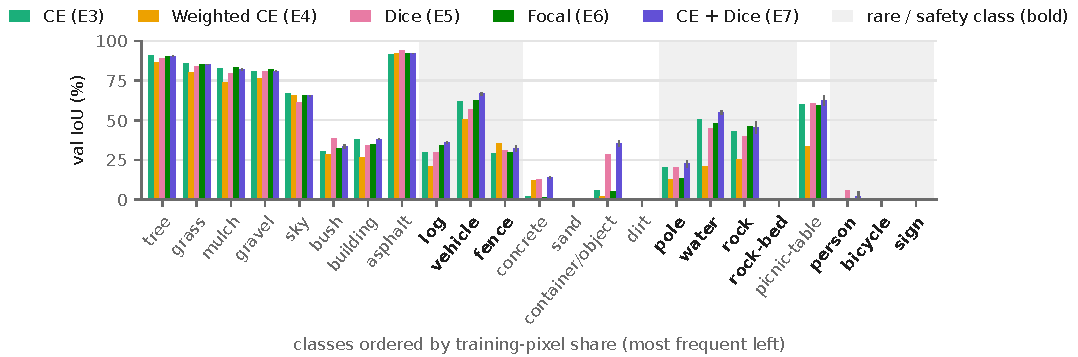
\includegraphics[width=\linewidth]{../results/figures/per_class_iou_losses.pdf}
  \caption{Per-class validation IoU by loss on DeepLabV3+/ResNet-50 (best
  epoch of each run), classes sorted by training frequency. Dice-based losses
  lift rare and mid-frequency classes without costing frequent ones; weighted
  CE lowers nearly every class.}
  \label{fig:perclass}
\end{figure}

\subsection{ImageNet Pretraining and Seed Variance}
\label{sec:res_pretrain}

Training the selected configuration from random initialization (E8) cost
5.7 points of validation mIoU (44.2$\to$38.5\%; 6.1 points GT-present). The
loss falls almost entirely on rare and mid-frequency objects (rock
43$\to$27\%, log 36$\to$25\%, container 37$\to$2\%, bush 32$\to$19\%, fence
33$\to$20\%), while frequent surfaces such as grass, asphalt, and gravel match
the pretrained model. E8 trails E7 at every epoch, by about 10 points early
and about 5 late, and ends at a higher training loss (0.43 vs.\ 0.33). The
gap was still narrowing, so this measures the benefit of pretraining under a
25-epoch budget, not at convergence.

\textbf{How noisy are these comparisons?} Two sources of noise matter. First,
validation mIoU fluctuates by 1--2 points from epoch to epoch after about
epoch 15 (Fig.~\ref{fig:curves}), and picking the best of 25 epochs rewards
single-epoch spikes. E3's 43.3\%, E7's 44.2\%, and E8's 38.5\% all sit one to
two points above the level each run settles at. Second, only one seed rerun
finished (Section~\ref{sec:compute}). The two seeds of CE+Dice differ by
1.0 point at their best epochs and by 2.3 points averaged over their last
five epochs (42.4 vs.\ 44.7\%), but by only 0.8 points on GT-present mIoU
(46.6 vs.\ 47.4\%). Much of the noise in the headline metric thus comes from
sporadic predictions of classes absent from validation. On the steadier
measure (GT-present, last-five-epoch mean) the ranking is: Dice (46.7) $\approx$
CE+Dice (46.6, 47.4) $>$ CE (43.5) $\approx$ focal (43.1) $>$ U-Net/R50 (41.4)
$\approx$ U-Net/R18 (40.6) $\approx$ no pretraining (40.5) $>$ weighted CE
(36.6). The Dice-based losses' gain over CE (about 3 points), the
pretraining gain (about 6), and weighted CE's loss (about 7) clearly exceed seed
noise. The encoder effect (0.8), CE+Dice versus Dice, and focal versus CE do
not. The decoder effect (2.1) is likely real but not by a wide margin. With
two seeds of one configuration these are rough bounds, not confidence
intervals.

\begin{figure}[t]
  \centering
  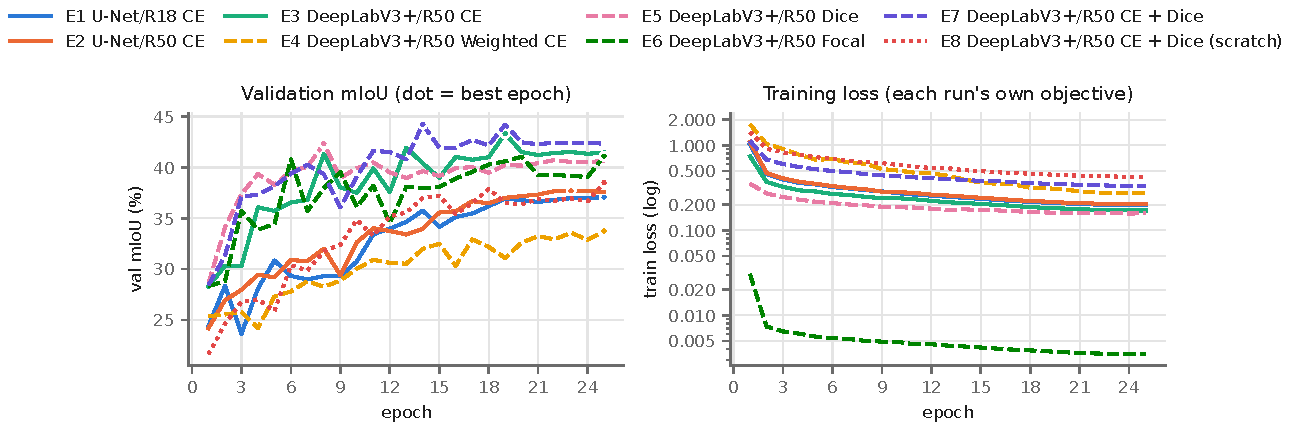
\includegraphics[width=\linewidth]{../results/figures/training_curves.pdf}
  \caption{Training loss and validation mIoU per epoch. After about epoch 15
  validation mIoU fluctuates by 1--2 points, so best-epoch selection favors
  single-epoch spikes. The run without pretraining (E8) trails its pretrained
  counterpart at every epoch, by about 10 points early and 5 points late.}
  \label{fig:curves}
\end{figure}

\subsection{Test Results and the Validation-to-Test Gap}
\label{sec:res_test}

On test, the selected CE+Dice model reaches 37.7\% mIoU, against 37.0\% for
CE (E3), 34.0--34.2\% for the U-Nets, and 32.2\% without pretraining
(Table~\ref{tab:main}). The ordering of architectures and of pretraining
matches validation, but CE+Dice's lead over CE shrinks to 0.7 points, within
seed noise, and CE is ahead on pixel accuracy, group mIoU, and rock. All
models lose 3--8 points of mIoU and 14--16 points of pixel accuracy from
validation to test (90--91\% to 74--77\%). The loss is almost entirely the
\emph{creek} sequence: it is 43\% of test pixels but produces 79--81\% of
every model's test errors, and it contains all of the test split's water and
rock-bed. Without creek, test mIoU is 49.3\% for CE+Dice, 47.9\% for CE,
43.5--44.3\% for the U-Nets and E8, and pixel accuracy is 90--92\%, on par
with validation. The validation-to-test gap is thus one unseen scene, not a
uniform drop, and is analyzed in Section~\ref{sec:error}. Our test mIoU is
above the RUGD baselines (31.8--32.2\%), though protocols differ
(Table~\ref{tab:main} footnote).

\subsection{Traversability Groups}
\label{sec:res_groups}

Mapping to six groups raises test mIoU from 37.7\% to 60.0\% for CE+Dice
(62.7\% for CE). Group IoU is high for obstacle (84\%), sky (82\%), and
vegetation (77\%), moderate for smooth (54\%) and rough ground (57\%), and
near zero for water (6\%). Coarsening helps most where fine-class errors stay
within a group, such as gravel versus rock-bed or grass versus bush, but
cannot help water, whose errors cross into the ground groups
(Section~\ref{sec:error}). CE's higher group mIoU comes mainly from rough
ground (67\% vs.\ 57\%), where CE+Dice labels more of creek's rock-bed as
smooth-ground mulch.

\subsection{Cross-Dataset Test on RELLIS-3D (Stretch Goal)}
\label{sec:res_rellis}

Zero-shot on the 1,672-frame RELLIS-3D test split, CE+Dice reaches 43.4\%
group mIoU with \emph{mud} ignored (43.6\% with mud scored as rough ground;
CE: 42.9\%), a drop of 16.6 points from its 60.0\% on RUGD test. The drop is
uneven. Sky (95\%) and vegetation (85\%) transfer, and even improve, since
they dominate RELLIS-3D frames (84\% of labeled pixels). Obstacles fall to
53\%, smooth ground to 25\%, and rough ground (\emph{rubble}, under 0.1\% of
pixels) and water (2\%) essentially fail. RELLIS-3D's dirt and asphalt are
predicted as vegetation or obstacle as often as ground (37\% recall), and its
puddles mostly as vegetation (49\%). The model's notion of ``ground'' is tied
to RUGD's mulch-and-gravel trails, and the safety-relevant groups are the
ones that transfer worst.

\section{Error Analysis}
\label{sec:error}

% All analyses use TEST predictions of the final model (E7 seed 1) and of the CE
% winner (E3); no decision in this section feeds back into model selection.

\subsection{Confusion Structure}

The row-normalized test confusion matrix of the final model
(Fig.~\ref{fig:confusion}) has five dominant off-diagonal patterns.
(i)~\emph{Water} is recalled only 6\% of the time: 54\% of its pixels are
predicted as \emph{mulch} and 22\% as \emph{grass}. (ii)~\emph{Rock-bed} goes
to mulch (41\%) or gravel (39\%). (iii)~\emph{Bush} splits between grass (36\%)
and tree (32\%). (iv)~Small obstacles are absorbed by their surroundings:
\emph{sign} (57\%) and \emph{pole} (29\%) are predicted as tree, \emph{person}
as tree, vehicle, or picnic-table. (v)~\emph{Dirt} goes to mulch (33\%) and
grass (21\%). Overall, 61\% of misclassified test pixels cross a traversability
group, and the most consequential crossing is safety-relevant: in the group
confusion, 55\% of water pixels are labeled \emph{smooth ground} and 34\% of
rough ground is also labeled smooth ground. A planner trusting these labels
would treat the creek as an easy trail.

\begin{figure}[t]
  \centering
  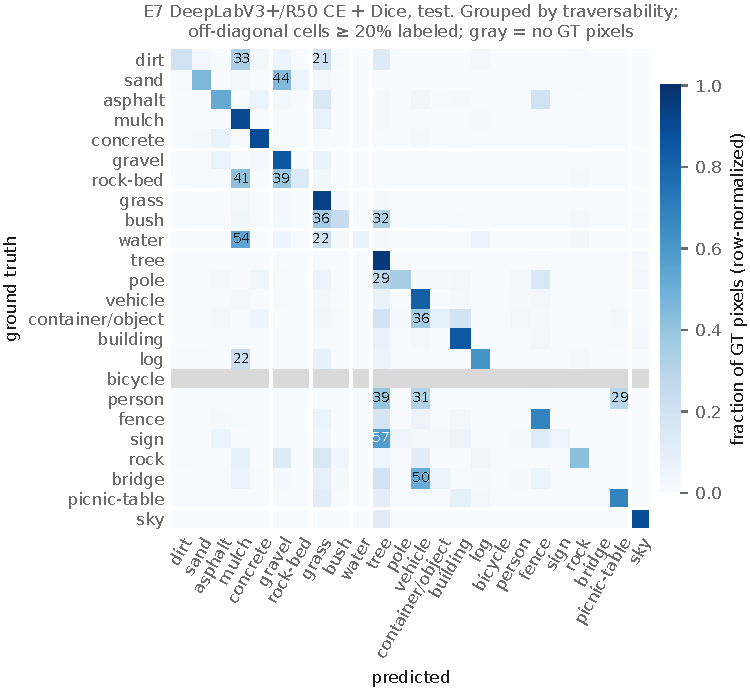
\includegraphics[width=\linewidth]{../results/figures/confusion_e7_ce_dice_s1_test.pdf}
  \caption{Row-normalized confusion matrix of the final model on RUGD test,
  classes ordered by traversability group. Water and rock-bed collapse into
  mulch and gravel; bush splits between grass and tree; thin objects are
  absorbed by \emph{tree}.}
  \label{fig:confusion}
\end{figure}

\subsection{Hardest Frames and Sequences}

Per-sequence test mIoU of the final model is 44.4\% on \emph{park-1}, 36.2\%
on \emph{trail-13}, 29.8\% on the motion-blurred \emph{trail-7}, and 15.0\% on
\emph{creek}, the order the RUGD authors anticipated~\cite{wigness2019rugd}.
The sequences fail differently. Trail-7 and trail-13 reach 92\% pixel accuracy:
their low mIoU comes from rare classes that occur in few frames, and 88--89\%
of their errors cross groups, mostly at obstacle/ground and tree/sky
transitions (logs against mulch, canopy gaps). Creek reaches only 56\% pixel accuracy. Its stream
is shallow, clear water over brown stones (Fig.~\ref{fig:gallery}, top rows),
which no training scene resembles. The model labels it by what shows through:
mulch-colored bed, with the surrounding cobbles as gravel or mulch. Both CE and
CE+Dice fail the same way, so the Dice term's validation gain on water (50$\to$56\%) does not transfer to
a stream. Logs,
by contrast, are segmented well on test by both models (48\% IoU), including
fallen trunks in trail-7 and a root ball in park-1.

The worst single frame (Fig.~\ref{fig:best_worst}, bottom) is a close-up of
leaves labeled entirely as \emph{bush}. The model predicts tree, mulch, and
rock. This is less a model error than an ambiguity of the coarse polygon
labels: at this distance, branch leaves and bush leaves are indistinguishable.

\begin{figure*}[t]
  \centering
  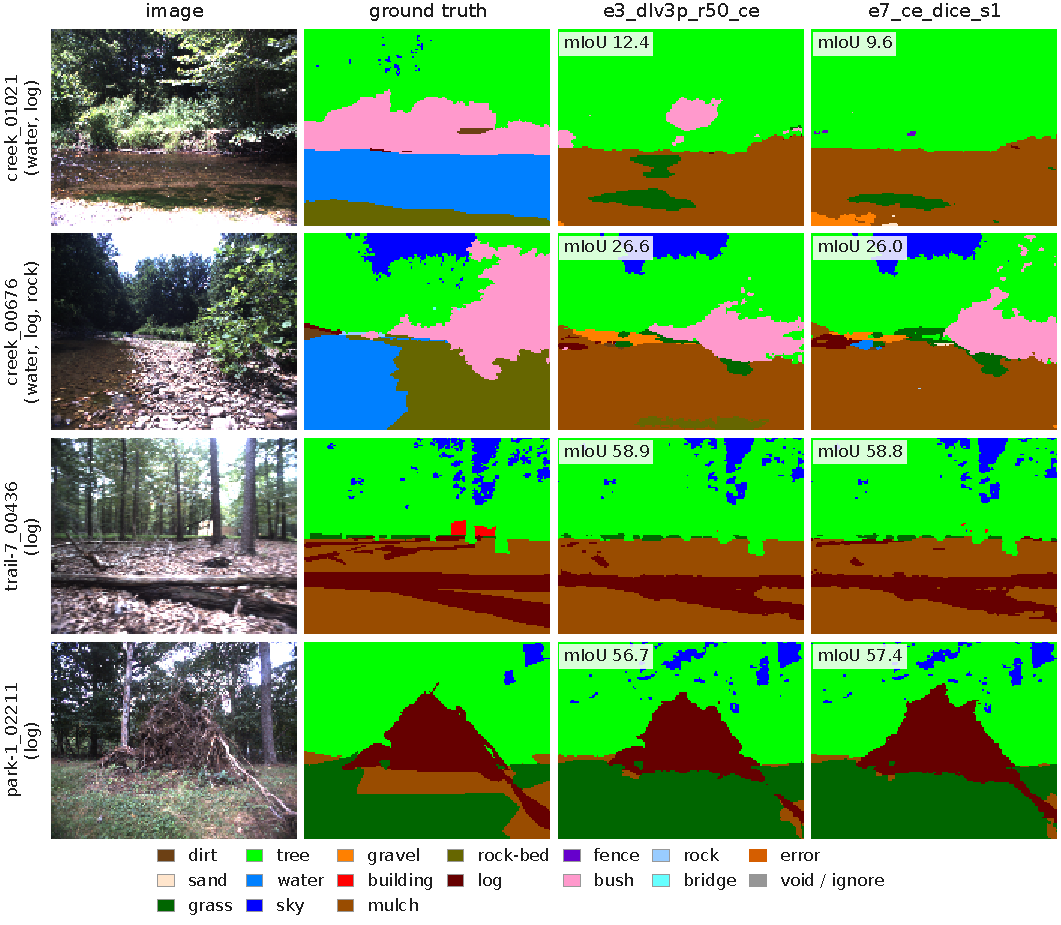
\includegraphics[width=0.82\textwidth]{../results/figures/compare_e3_dlv3p_r50_ce_vs_e7_ce_dice_s1_test.pdf}
  \caption{CE (E3) vs.\ CE+Dice (E7, seed 1) on test frames containing water,
  log, or rock, with per-frame mIoU. Rows 1--2 (creek): both models label the
  clear, shallow stream as mulch and the cobble bed (\emph{rock-bed}, olive) as
  mulch or gravel. Rows 3--4: logs are segmented well by both. In the official
  palette, \emph{concrete} and \emph{rock-bed} have nearly identical colors;
  no concrete appears in these frames.}
  \label{fig:gallery}
\end{figure*}

\begin{figure}[t]
  \centering
  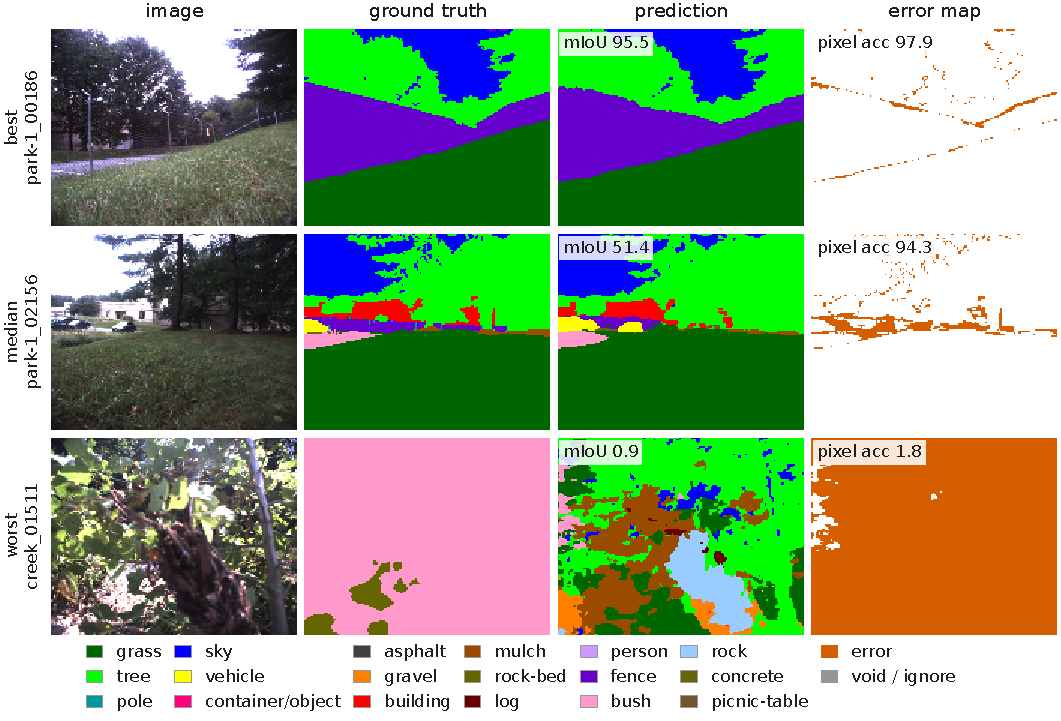
\includegraphics[width=\linewidth]{../results/figures/gallery_e7_ce_dice_s1_test.pdf}
  \caption{Best, median, and worst test frames of the final model by per-frame
  mIoU. Errors in good frames sit on class boundaries (fence edges, tree/sky
  transitions); the worst frame is a leaf close-up labeled \emph{bush}.}
  \label{fig:best_worst}
\end{figure}

\subsection{Boundary Ambiguity}

Excluding a 3-pixel band around label boundaries (at $384^2$), which holds
15\% of test pixels, raises the final model's test mIoU from 37.7\% to 40.8\%;
pixel accuracy is 79\% in the interior and 61\% in the band. Yet the band
holds only 26\% of test errors (13\% at 1\,px, 34\% at 5\,px). On validation,
by contrast, the same band holds 53\% of errors. Where the model recognizes the
scene, as in validation, most residual error lies at ambiguous transitions
(grass/mulch, bush/tree), consistent with the coarse polygon labels. On
test, most error comes from whole regions misrecognized in creek, which no
boundary tolerance can recover. The pattern is the same for every model
(Table~\ref{tab:main} models: 24--27\% of test errors in the 3\,px band).

\subsection{Classes the Data Cannot Support}

\emph{Bridge} illustrates a failure that no loss function can fix: with zero
training pixels, its roughly 4.6\,M native-resolution test pixels must be
assigned to some other class. The final model predicts \emph{vehicle} for 50\%
of them (CE: 71\%), then tree (19\%) and grass (8\%), the nearest learned
large man-made structure and its surroundings. Its IoU is 0 by construction.
\emph{Bicycle} is absent from test, and the final model predicts it on no test
pixel, so it does not enter the test mIoU.

\section{Discussion and Future Work}
\label{sec:discussion}

% Risk table (Section VII-A) defined here so the full-width float lands before the references.
\begin{table*}[t]
  \centering
  \caption{Updated risk and ethics reflection: anticipated (A) and newly emerged (N) issues and how each was handled.}
  \label{tab:risks}
  \footnotesize
  \begin{tabular}{@{}p{2.9cm} p{6.7cm} p{7.2cm}@{}}
    \toprule
    Issue & What emerged & How it was managed \\
    \midrule
    Class imbalance (A) &
      Worse than expected: 6,382:1 between \emph{tree} and \emph{sign};
      safety classes 1.1\% of training pixels. &
      Four imbalance-aware losses vs.\ CE; train-only median-frequency weights,
      clipped at 50; per-class IoU reported. \\
    Split shift (N) &
      \emph{Bridge} only in test; validation lacks four classes; test is
      hazard-heavy (safety classes 10.3\% vs.\ 1.1\%), driven by \emph{creek};
      val closer to train than to test. &
      Official split kept for comparability; \emph{bridge} excluded from headline
      mIoU but reported; val and test reported separately; test per-class IoU;
      test guarded by a flag and used once. \\
    Leakage and labels (A) &
      Labeled frames are near-duplicates (every fifth video frame); coarse
      polygons, wires labeled \emph{tree}, sticks labeled \emph{log},
      near-identical concrete/rock-bed colors. &
      Sequence-level split verified (20-frame discrepancy with~\cite{wigness2019rugd}
      disclosed); boundary-band analysis (Section~\ref{sec:error}); palette
      caveat in captions. \\
    Compute (A) &
      Apple M1 Pro too slow at $512^2$ and unstable in validation; Colab T4
      sessions capped at about 12\,h. &
      $384^2$/25 epochs for \emph{all} runs; mixed precision on T4; per-epoch
      checkpoints on Drive with automatic resume (Section~\ref{sec:compute}).
      Outcome: quota ran out before 3 of 4 seed reruns, and four checkpoints
      were lost to a storage mishap; disclosed, and the selected configuration's
      replicate used for test. \\
    Domain shift (A) &
      Different vehicle, viewpoint, and label mix in RELLIS-3D; \emph{mud} has
      no RUGD counterpart. &
      Group map fixed before evaluation; mud ignored in the headline score with
      a sensitivity check; zero-shot only. Outcome: group mIoU fell from 60.0\% to
      43.4\%; ground and water transfer worst (Section~\ref{sec:res_rellis}). \\
    Safety, dual use, licensing &
      Rare hazards are the most likely misses; Army-funded data;
      RELLIS-3D is CC BY-NC-SA 3.0. &
      Rare-class IoU reported; models presented as research artifacts;
      non-commercial use; no redistribution of images. \\
    \bottomrule
  \end{tabular}
\end{table*}

\subsection{What Worked}

Adding a Dice term to the loss was the most useful single change: about 3
points of GT-present validation mIoU over CE (Section~\ref{sec:res_pretrain}),
concentrated on water, log, container, and concrete, with frequent classes
and pixel accuracy unchanged. Because Dice normalizes per class over the
batch, a rare class's gradient no longer scales with its pixel count, which
is the imbalance a pixel-averaged loss suffers from. ImageNet pretraining was
the largest single factor (about 6 points) and mattered most for the same
rare objects. The DeepLabV3+ decoder helped moderately (about 2 points),
mainly on objects whose extent needs multi-scale context, such as vehicles
and picnic tables.

\subsection{What Did Not Work}

Median-frequency weighted CE hurt across the board ($-9.6$ validation mIoU,
$-5.0$ pixel accuracy): weights up to 50 made the model over-predict rare
classes, so their false positives grew faster than their true positives.
Deepening the encoder from ResNet-18 to ResNet-50 bought less than seed
noise. \emph{Dirt}, \emph{sign}, and \emph{person} stayed near zero under
every loss: dirt is 0.13\% of training pixels and visually close to mulch and
sand, and signs and people are tiny at $384^2$. Best-epoch selection on a
noisy, incomplete validation split was itself a weakness. Under our
pre-registered rule, Dice alone looked 2 points worse than CE+Dice, when on
the classes validation actually contains the two are tied. The validation-to-test gap (7.5 points for the final model) was
concentrated in one scene: creek, whose clear stream the model reads as mulch,
caused 80\% of test errors, and without it test mIoU (49.3\%) matches
validation. A validation split with no flowing water could not warn us. Some limitations
are structural rather than methodological. Validation lacks four classes, so
model selection cannot reward improvements on \emph{sand}, \emph{rock-bed},
\emph{bicycle}, or \emph{bridge}, and its class mix is closer to training
than to test, so it is an optimistic proxy. The test split's rare hazards come
almost entirely from one sequence, which makes their IoU a high-variance
estimate. The reduced $384^2$, 25-epoch schedule
(Section~\ref{sec:compute}) limits thin-structure accuracy and may understate
what each configuration can reach. With two seeds for one
configuration (the other planned reruns did not fit the free GPU quota),
we can bound run-to-run noise only roughly, and the test results for the
selected configuration come from its seed-1 replicate.

\subsection{Future Work}

(i)~Train at native resolution or with sliding-window inference to recover
thin obstacles. (ii)~Re-split or use sequence-level cross-validation so that
validation covers every trainable class and matches the test class mix.
(iii)~Exploit temporal consistency across RUGD's video frames. (iv)~Compare
transformer backbones and group-aware objectives such as
GA-Nav~\cite{guan2022ganav}. (v)~Calibrate uncertainty so a planner can treat
low-confidence water or obstacle pixels conservatively. (vi)~Fine-tune on a
small RELLIS-3D subset, drawn by sequence rather than by frame, to measure how
much target data closes the cross-dataset gap, which was largest for ground
and water (Section~\ref{sec:res_rellis}). (vii)~Add water-specific cues, such
as specular-reflection or temporal-flicker features, or a small labeled set
of streams, since appearance alone failed on clear, shallow water.

\section{Ethical Considerations}
\label{sec:ethics}

\textbf{Representativeness and bias.} RUGD covers a few parks, trails, a
creek, and a village, recorded by one small robot with a camera under 25\,cm
above the ground~\cite{wigness2019rugd}. Season, geography, weather, and time
of day are narrowly sampled; snow, desert, night, and heavy rain are absent,
and there is no \emph{mud} class. A model trained here may look reliable on
similar trails yet fail silently on unseen terrain or on the higher viewpoint
of a full-size vehicle. A segmentation model has no demographic attributes, but
the same principle applies: error rates differ across environments, and
under-represented environments carry the least evidence. Even within RUGD,
test hazards come almost entirely from one creek sequence, and people cover
only 0.012\% of training pixels, so rare-class and \emph{person} IoU are weak
evidence and must not be read as evidence of pedestrian safety. We therefore
report per-class and per-sequence results, not only mIoU.

\textbf{Safety, dual use, licensing, and privacy.} The costliest errors are
missed hazards, such as water labeled as drivable ground, and these are the
rarest classes, so a high mIoU can hide them. Our models are research artifacts
evaluated offline, \emph{not} safety systems, and any driver-assist use would
need independent validation, calibrated uncertainty, redundant sensing, and an
advisory-only role. Both datasets involved the U.S. Army Research
Laboratory~\cite{wigness2019rugd,jiang2021rellis}, and off-road autonomy has
military as well as civilian uses; we use only openly published methods and
data. RELLIS-3D is licensed CC BY-NC-SA 3.0~\cite{jiang2021rellis}, so anything
derived from it is non-commercial and shared alike; neither dataset's images
are redistributed. No legible faces or plates appeared in inspected frames,
our figures avoid identifiable people, and demo photographs are stripped of
EXIF/GPS metadata and framed to exclude people and license plates.

\subsection{Updated Risk and Ethics Reflection}
\label{sec:reflection}

Table~\ref{tab:risks} compares the risks anticipated in our proposal with
what emerged and how each was handled.

\begin{table*}[t]
  \centering
  \caption{Updated risk and ethics reflection: anticipated (A) and newly emerged (N) issues and how each was handled.}
  \label{tab:risks}
  \footnotesize
  \begin{tabular}{@{}p{2.9cm} p{6.7cm} p{7.2cm}@{}}
    \toprule
    Issue & What emerged & How it was managed \\
    \midrule
    Class imbalance (A) &
      Worse than expected: 6,382:1 between \emph{tree} and \emph{sign};
      safety classes 1.1\% of training pixels. &
      Four imbalance-aware losses vs.\ CE; train-only median-frequency weights,
      clipped at 50; per-class IoU reported. \\
    Split shift (N) &
      \emph{Bridge} only in test; validation lacks four classes; test is
      hazard-heavy (safety classes 10.3\% vs.\ 1.1\%), driven by \emph{creek};
      val closer to train than to test. &
      Official split kept for comparability; \emph{bridge} excluded from headline
      mIoU but reported; val and test reported separately; test per-class IoU;
      test guarded by a flag and used once. \\
    Leakage and labels (A) &
      Labeled frames are near-duplicates (every fifth video frame); coarse
      polygons, wires labeled \emph{tree}, sticks labeled \emph{log},
      near-identical concrete/rock-bed colors. &
      Sequence-level split verified (20-frame discrepancy with~\cite{wigness2019rugd}
      disclosed); boundary-band analysis (Section~\ref{sec:error}); palette
      caveat in captions. \\
    Compute (A) &
      Apple M1 Pro too slow at $512^2$ and unstable in validation; Colab T4
      sessions capped at about 12\,h. &
      $384^2$/25 epochs for \emph{all} runs; mixed precision on T4; per-epoch
      checkpoints on Drive with automatic resume (Section~\ref{sec:compute}). \\
    Domain shift (A) &
      Different vehicle, viewpoint, and label mix in RELLIS-3D; \emph{mud} has
      no RUGD counterpart. &
      Group map fixed before evaluation; mud ignored in the headline score with
      a sensitivity check; zero-shot only. \todo{update with outcome} \\
    Safety, dual use, licensing &
      Rare hazards are the most likely misses; Army-funded data;
      RELLIS-3D is CC BY-NC-SA 3.0. &
      Rare-class IoU reported; models presented as research artifacts;
      non-commercial use; no redistribution of images. \\
    \bottomrule
  \end{tabular}
\end{table*}


\bibliographystyle{IEEEtran}
\bibliography{refs}

\end{document}
